\documentclass{article}
\usepackage{graphicx}
\usepackage[margin=1.5cm]{geometry}
\usepackage{amsmath}

\begin{document}

\title{Tuesday Reading Assessment: Chapter 1}
\author{Prof. Jordan C. Hanson}

\maketitle

\section{Basic Logic Operations}

\begin{enumerate}
\item Observe Fig. \ref{fig:oper1} below.  
\begin{figure}[ht]
\centering
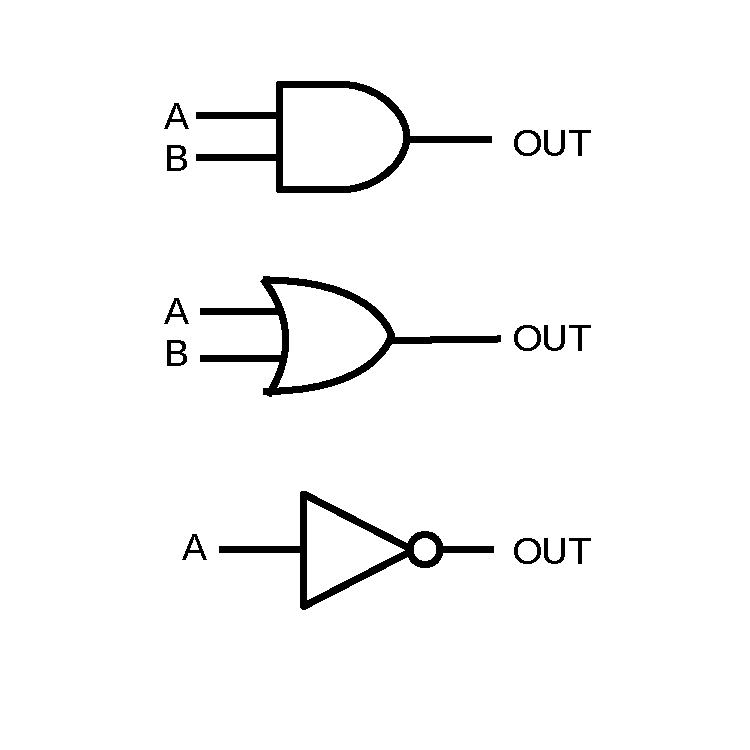
\includegraphics[width=0.25\textwidth]{Operators3.pdf}
\caption{\label{fig:oper1} Three basic logic operations.}
\end{figure}
If the inputs A and B can either be HIGH or LOW, list all possible combinations of inputs of A and B. \\ \vspace{1cm}
\item Which combinations of A and B produce a HIGH output on the top gate? \\ \vspace{1cm}
\item Which combinations of A and B produce a HIGH output on the middle gate? \\ \vspace{1cm}
\item What is the output of the bottom gate if the input A is LOW?
\end{enumerate}

\end{document}
